\subsubsection{Measurement Operations}
\label{sec:geo_measure_ops}

To access the map operations, click the measurement symbol \includegraphics[width=0.5cm,frame]{../../data/icons/measure.png}, then the following operations are available:

\begin{itemize}
 \item Copy All Texts: Copies measurement data as text to the clipboard
 \item Delete All: Removes all measurements
\end{itemize} 

\begin{figure}[H]
    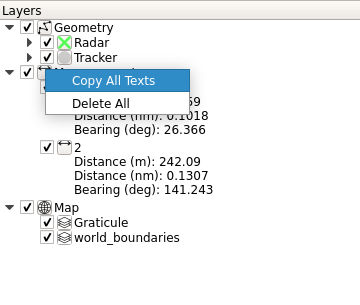
\includegraphics[width=8cm,frame]{figures/geoview_measure_ops.png}
  \caption{Geographic View measurement layer operations}
\end{figure}

A copied measurement text looks as follows:

\begin{lstlisting}
1
Distance (m): 188.59
Distance (nm): 0.1018
Bearing (deg): 26.366
Point1: 36.56370614, 15.74786596
Point2: 36.56522404, 15.74880269

2
Distance (m): 242.09
Distance (nm): 0.1307
Bearing (deg): 141.243
Point1: 36.55986876, 15.72751885
Point2: 36.55817286, 15.72921376
\end{lstlisting}
